
\chapter{Modèle de polymères}
\label{polymerevalidation}

\cleardoublepage

{\Large\textbf{{Modèle de polymères}}}\\

\lettrine[loversize=0.6,lraise=0.1,findent=0.5em,nindent=0em]{D}{}ans ce chapitre, nous détaillons l'élaboration d'un modèle de polymères que nous utiliserons par la suite pour aborder la translocation. Nous avons opté pour un modèle gros grain et discutons de sa pertinence, des potentiels utilisés ainsi que des conditions dans lesquelles ont lieux les simulations. Ce modèle est ensuite testé et comparé à la théorie dans des situations statiques, dynamiques et de traction.\\

\minitoc

\begin{center}
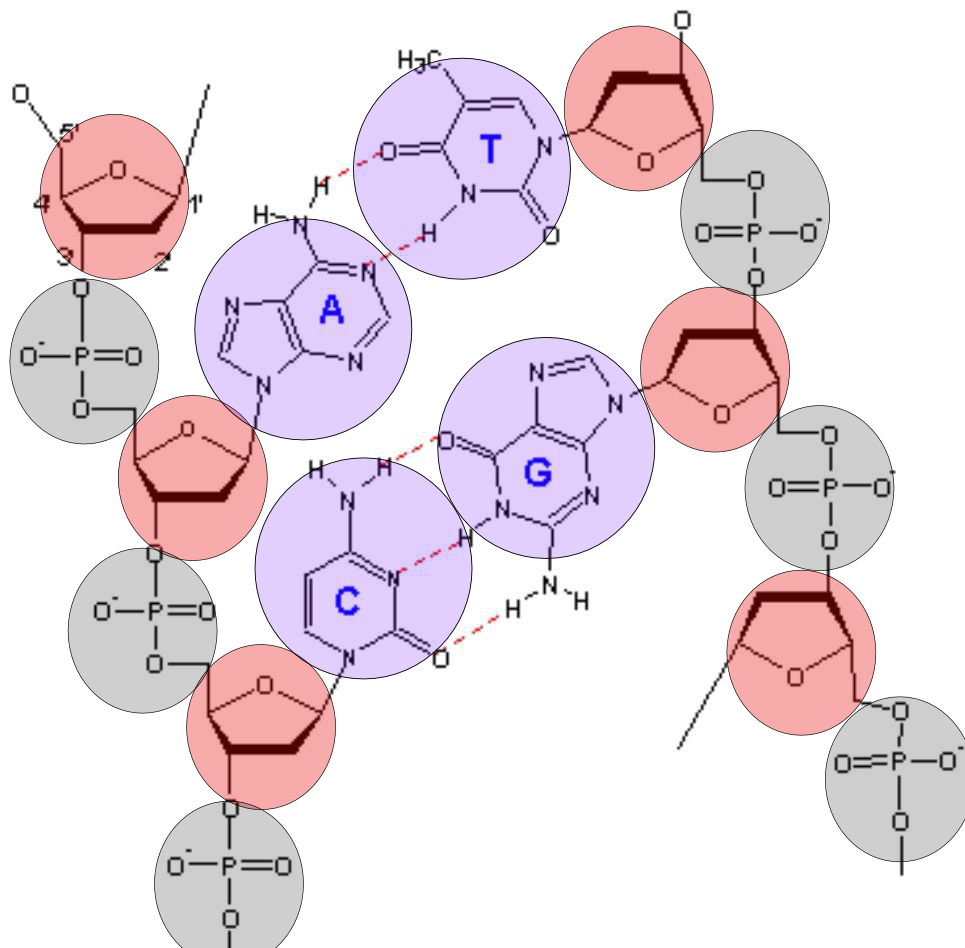
\includegraphics[width=0.7\textwidth]{coarsegraining.png}
\end{center}

\cleardoublepage







\section{Construction d'un modèle gros grain}

Comme nous l'avons vu dans le paragraphe précédent, l'utilisation de modèles gros grains, combinée à la dynamique moléculaire, permet de modéliser la translocation. Nous avons choisi cette méthode pour étudier le problème à une échelle qui n'a, à notre connaissance, pas encore était explorée. Nous nous proposons d'étudier un modèle suffisamment simple pour obtenir des résultats statistiquement pertinents, mais également suffisamment élaboré pour refléter certaines structures de l'ADN.

\subsection{Pertinence du modèle}
Avant même d'aborder le problème de la translocation, il est important de souligner la pertinence de l'utilisation de modèles gros grains et de la dynamique moléculaire dans l'étude de l'ADN. Comme nous l'avons signalé précédemment, une description du polymère prenant en compte tous les atomes est prohibitive en temps de calcul et inutile pour une analyse statistique complète. Il est donc nécessaire de rassembler plusieurs atomes dans un ensemble ( un grain) cohérent et de définir proprement les interactions entre ces ensembles. Rappelons que l'ADN est composé d'une chaîne principale, succession de phosphates et de sucres et de bases azotées greffées de manière latérale sur les sucres. Ces trois éléments sont des candidats idéaux pour une description de l'ADN constituée de trois types de grains, comme présenté sur la figure \ref{coarsegraindna}.

\begin{figure}[H]
\begin{center}
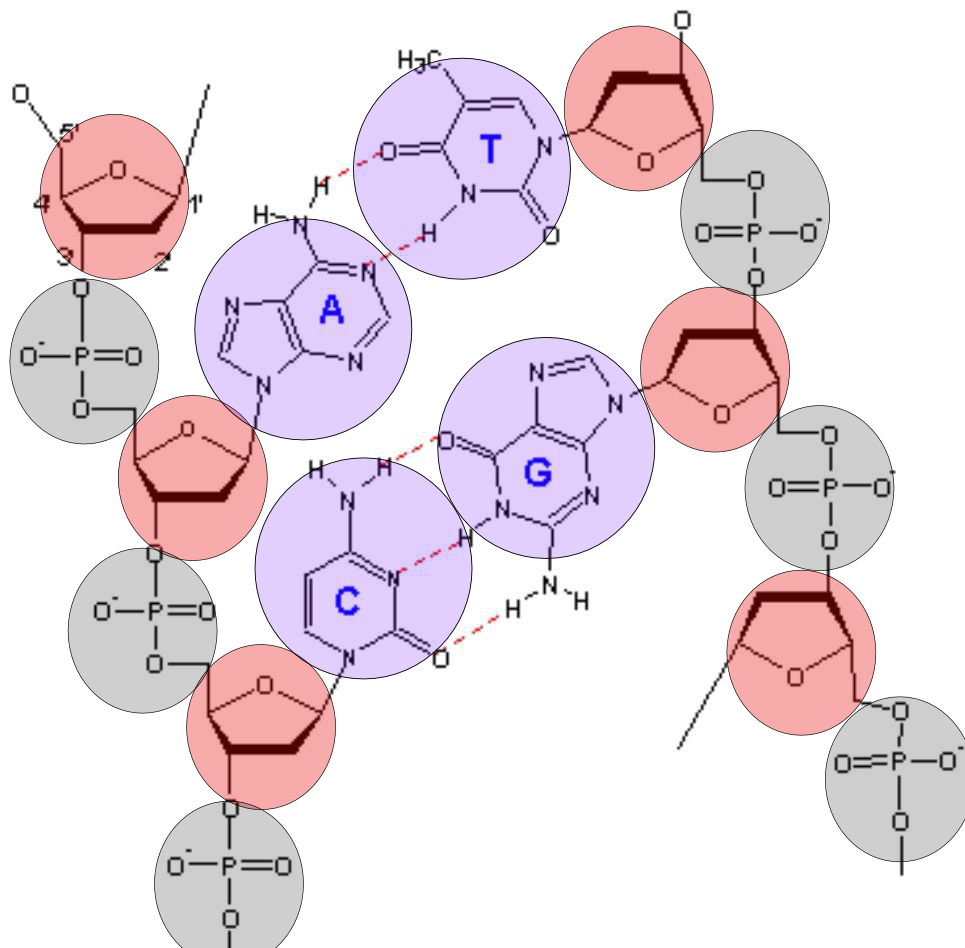
\includegraphics[width=0.65\textwidth]{coarsegraining.png}

\caption[Modèle gros grains]{Représentation gros grain de l'ADN. Trois types de grains représentant les phosphates, sucres et bases azotées composent un modèle d'ADN. De tailles proches, ces grains sont définis à partir d'éléments rigides et liés de manière covalente simple. Une fois la structure de grain définie, il faut définir leurs interactions.}
\label{coarsegraindna}
\end{center}
\end{figure}


En effet, plusieurs éléments justifient ce choix. Phosphate, sucres et bases azotées sont de tailles du même ordre de grandeur. Ils sont individuellement très peu déformables, de par sa géométrie pour le phosphate et par la présence de cycles rigides pour les sucres et les bases azotées. Les liaisons covalentes simples permettant une libre rotation sont situées entre ces grains. Une fois les grains choisis, il faut définir la manière dont ils interagissent entre eux. On définit donc des potentiels d’interaction. Pour l'ADN, on peut distinguer trois types de potentiels à définir: les interactions non spécifiques, la torsion au sein de la chaîne et les interactions entre bases azotées. Ces potentiels sont définis à partir d'étalons de distance ($\sigma$ et $R_0$) et d'énergie ($\epsilon$) qui traduisent les propriétés physiques du polymère. A partir de ces valeurs, on peut créer des échelles a-dimensionnées de temps, température, viscosité, force... On parle d'unités de Lennard-Jones. On discutera de la valeur de ces paramètres après avoir justifié les potentiels utilisés.


\subsection{Potentiels d'interaction}

\subsubsection{Interactions non spécifiques}

Il existe deux types d'interactions non spécifiques: les contacts entre grains et leurs liaisons. 

\begin{figure}[H]
\begin{center}
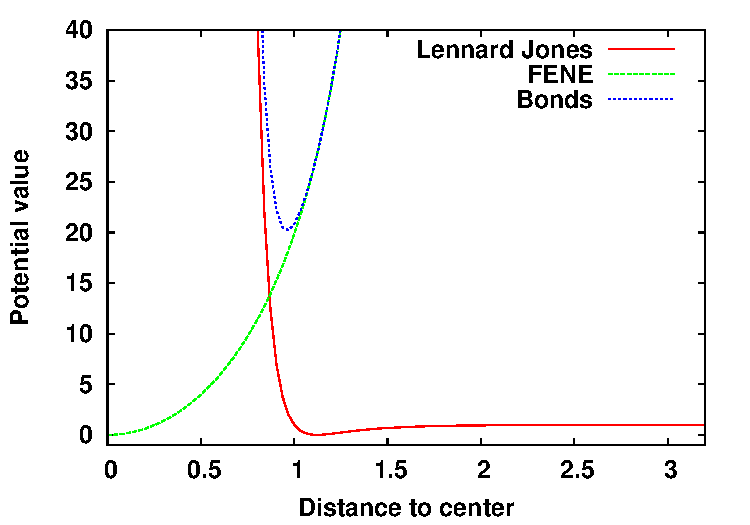
\includegraphics[width=0.75\textwidth]{nonspec.pdf}

\caption[Potentiels stériques]{interactions non spécifiques pour un modèle gros grain de bio-polymère. Le potentiel de Lennard-Jones représente les interactions de contacts stériques et de Van der Waals entre grains. Combiné avec un potentiel de type FENE, on obtient une bonne représentation de liaison covalente simple.}
\label{nonspecificinterac}
\end{center}
\end{figure}


Pour les contacts, nous avons choisi d'utiliser un potentiel de type Lennard-Jones (LJ) \cite{Jones1924}, très répandu dans la littérature du fait de son adéquation avec les résultats expérimentaux \cite{Bouanich1992}:

\begin{eqnarray}
U_{LJ}(r_{ij})= 4\epsilon_{ij} \left[\left(\frac{\sigma_{ij}}{r_{ij}}\right)^{12}-\left(\frac{\sigma_{ij}}{r_{ij}}\right)^{6}\right] + \epsilon_{ij} \text{ }, \text{ } U_{LJ}(r_{ij})=0 \text{ pour }  r_{ij}> 2^{1/6}\sigma_{ij}
\end{eqnarray}

\noindent $r_{ij}$ étant la distance entre les grains i et j, ce potentiel empêche l'interpénétration à faible distance. On définit une taille de grain $\sigma$ pour chaque type de grain, une taille moyenne est utilisée pour le contact de grains de tailles différentes ($\sigma_{ij}=\frac{\sigma_i+\sigma_j}{2}$). L'échelle d'énergie $\epsilon_{ij}$ sera dans notre cas toujours égal à $\epsilon$ quelque soient $i$ et $j$. ceci permettra de limiter le nombre de paramètres ajustables.

Les liaisons covalentes entre grains sont modélisées par un potentiel anharmonique de type FENE (Finitely Extensible Nonlinear Elastic) :
\begin{eqnarray}
U_{FENE}(r_{ij})= -15\epsilon \left(\frac{R_0}{\sigma_{ij}}\right)^2\text{ } \ln\left[1-\left(\frac{r_{ij}}{R_0}\right)^2\right]
\end{eqnarray}
Un développement limité montre le comportement harmonique à faible distance et le logarithme impose une extension maximale $R_0$ à la liaison, $R_0$ que nous avons pris égal à 1.5 la taille $\sigma$ moyenne des grains liés. Le potentiel FENE représentant la contribution attractive de la liaison covalente est utilisé en complément du potentiel de Lennard-Jones, répulsif à courte distance. Il en résulte une position d'équilibre très stable qui est caractéristique de la longueur de la liaison. Les potentiels des interactions non spécifiques sont tracés sur la figure \ref{nonspecificinterac}.

\subsubsection{Torsion et interactions entre bases}

Viennent ensuite les interactions spécifiques particulières à l'ADN. Au sein de la chaîne il y à une certaine rigidité qui peut être modélisée par un potentiel d'interaction à trois corps comme proposé par Linak, Tourdeau et Dorfman \cite{jchem}: 

\begin{eqnarray}
U_{BB}(\phi)= 12\epsilon \left( 1+cos(\phi)\right)^{2}
\end{eqnarray}

\noindent Avec $\epsilon$ une échelle d'énergie et $\phi$ l'angle formé dans l'axe Sucre-Phosphate-Sucre, la rigidité de la liaison est traduite par un angle d'équilibre de $\pi$, soit une chaîne droite, voir figure \ref{torsion}. La flexibilité de la chaîne est permise une dérivée second faible près de l'équilibre et un puit de potentiel assez large.

\begin{figure}[H]
\begin{center}
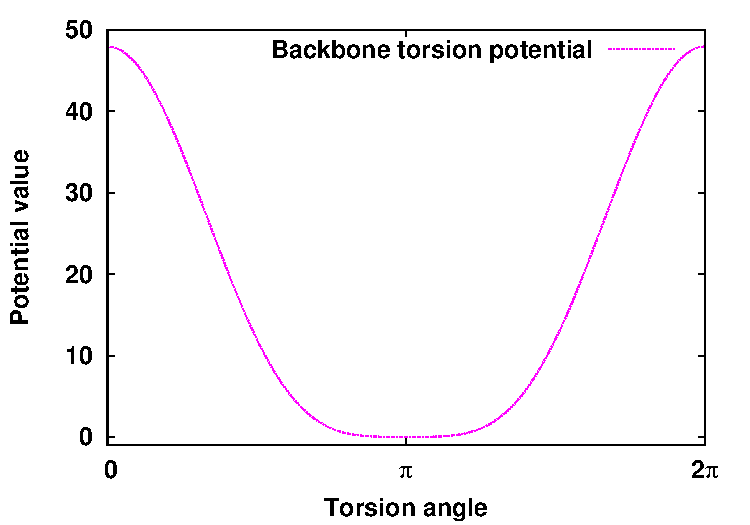
\includegraphics[width=0.7\textwidth]{backbone.pdf}

\caption[Potentiel de torsion]{La rigidité au sein de la chaîne peut être modélisée par un potentiel de torsion à trois corps. La position d'équilibre de $\pi$ favorise une chaîne linéaire mais le minimum peut prononcé, permet une certaine déformabilité pour les chaînes longues.}
\label{torsion}
\end{center}
\end{figure}

Parmi les interactions spécifiques, on identifie également les interactions entre bases azotées. Elles sont de deux types: liaisons hydrogènes et interactions orbitalaires directes ou croisées ($\pi$ stacking en anglais). Ces interactions peuvent (combinées à un potentiel de Lennard-Jones) être modélisées par le produit d'une fonction dépendante de la distance entre grains et d'une fonction caractéristique de leur orientation (avec un angle à définir). La figure \ref{hbonds} décrit un exemple de modélisation de ses interactions.


\begin{figure}[H]
\begin{center}
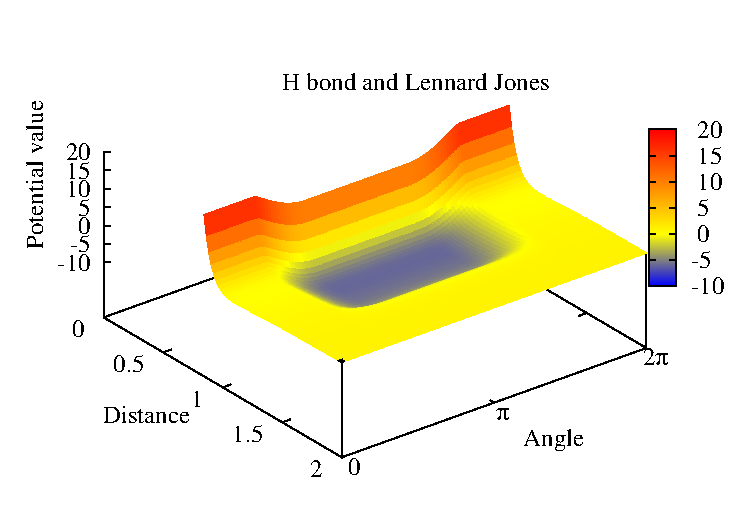
\includegraphics[width=0.9\textwidth]{bbhbonds.pdf}
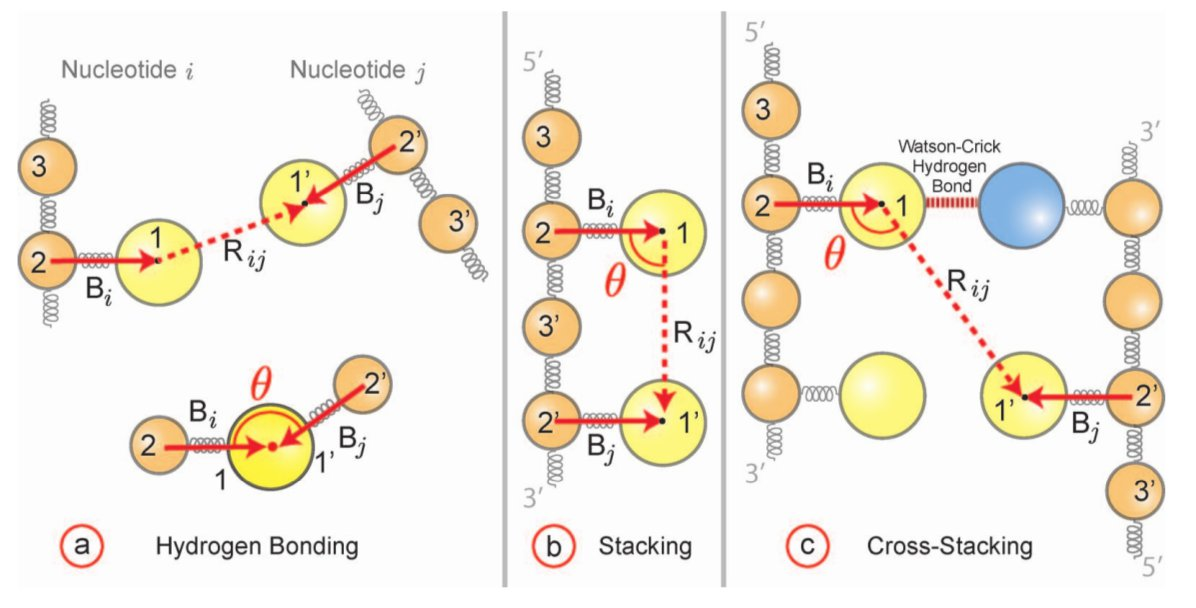
\includegraphics[width=0.9\textwidth]{specinterac.jpg}

\caption[Potentiels d'interaction spécifiques]{En haut: Exemple de potentiel permettant de décrire une liaison hydrogène. Le potentiel (auquel s'ajoute le potentiel de Lennard Jones) est modélisé par le produit d'une fonction caractéristique de l'éloignement des grains et d'une fonction représentant leur orientation. Le même type de potentiel peut être utilisé pour les interactions orbitalaires en définissant différemment l'angle de l'interaction. En bas: Exemple de définition d'angle \cite{jchem}.}
\label{hbonds}
\end{center}
\end{figure}

\subsubsection{Gains en coût de calcul}

Les potentiels décrits précédemment permettent de modéliser efficacement le comportement de l'ADN comme en attestent les travaux de Linak et al. \cite{jchem} qui décrivent l'ouverture d'épingles au sein de l'ADN ou le repliement d'un aptamère (petite séquence d'ADN synthétique capable de se fixer à un ligand spécifique). Cependant l'utilisation de potentiel élaborés augmente fortement le coût, en terme de calcul informatique, de résolution des trajectoires.

Ainsi, pour les potentiels simples à deux corps des interactions non spécifiques, il suffit de calculer la distance entre chaque couples de grains, une seule grandeur est calculée en une seule opération. On a alors un nombre de calculs à effectuer égal au nombre de paires possibles. Pour N grains on a alors un temps de calcul $\tau_c$ proportionnel à $N^2$ pour N grand comme le montre l'équation \ref{pairpot}.

\begin{eqnarray}
\tau_c(pairpotential) \propto \frac{N(N-1)}{2} \underset{N \rightarrow +\infty}{\sim} \frac{N^2}{2}
\label{pairpot}
\end{eqnarray}

On peut même utiliser pour N suffisamment grand des algorithmes plus efficaces basés sur l'utilisation de listes de plus proches voisins \cite{Vaidya1989} qui vont se comporter à l'infini en $O(Nln(N))$.

En ce qui concerne les potentiels à trois corps, le nombre de calculs nécessaires devient vite plus important. Ils nécessitent de définir un angle (il faut trois éléments pour cela). Le nombre d'opérations par rapport à une interaction non spécifique peut être identique, comme dans le cas du potentiel de torsion (uniquement le calcul de $cos(\theta)$ via un produit scalaire est nécessaire de par la symétrie du potentiel) ou doubler si le calcul de la distance est également nécessaire. On a alors un nombre de potentiels à calculer qui peut vite devenir prohibitif. Pour la torsion, le nombre de potentiels est lié au nombre de liaisons et va donc varier en $O(N)$. En ce qui concerne les interactions entre bases, avec un possible repliement du polymère et la création de structures en épingles, on a un nombre de potentiels à calculer proportionnel au nombre de triplets de grains représentant les bases et donc un temps de calcul décrit par l'équation \ref{3bodypot}, qui pourra éventuellement être amélioré par l'utilisation d'algorithmes de type liste de plus proches voisin, mais demeurant toujours extrêmement élevé.

\begin{eqnarray}
\tau_c(3bodypotential) \propto \frac{N(N-1)(N-2)}{6} \underset{+\infty}{\sim} \frac{N^3}{6}
\label{3bodypot}
\end{eqnarray}



Afin d'étudier la translocation de bio-polymères, nous allons utiliser des ADN simple brins et des chaînes relativement courtes, les potentiels d'interactions entre bases et de torsion en plus d'être gourmand en effort de calcul ne sont donc pas des plus pertinents. En effet, une chaîne courte représentera donc une tige rigide si on applique la torsion, on s'éloigne alors du problème réel. La différence de longueur de persistance pour un ADN simple brin reste limitée (de l'ordre de 1 à 2 bases), contrairement à la rigidité du double brin (longueur de persistance de l'ordre de 150 paires de bases) qui nécessite alors la prise en compte de la torsion. De plus nous n'avons pas pour objectif d'étudier les effets d'éventuelles épingles dans l'ADN sur la translocation, ce qui fait que des auto-interactions entre bases au sein du polymère ne sont pas non plus pertinentes.

Pour notre modèle de polymère, nous n'allons donc conserver que des interactions non spécifiques afin de créer un polymère simple mais structuré dans des proportions géométriquement proches de l'ADN. On aura uniquement des potentiels de type Lennard-Jones, éventuellement couplés à des potentiels de type FENE pour les liaisons covalentes entre grains.

\subsection{Conditions de simulation}

\subsubsection{Dynamique moléculaire et résolution des équations du mouvement}

Les potentiels choisis, il faut maintenant résoudre les trajectoires de translocation. Nous allons alors définir les conditions de simulation, les équations du mouvement à résoudre, les méthodes numériques utilisées et relier ce qui peut l'être aux conditions expérimentales.
Un fichier caractérisant le système ainsi qu'une liste d'instructions sont fournis à un solveur de dynamique moléculaire, LAMMPS \cite{lammps}, afin de réaliser nos simulations.

\subsubsection{Conditions thermodynamiques et équations du mouvement}



Pour résoudre nos trajectoires, nous nous plaçons dans l'ensemble canonique, nous travaillons donc avec un nombre de grains constant, un volume constant (avec des conditions aux limites périodiques) et température constante. La gravité, faible devant les autres grandeurs du problème n'est pas prise en compte.


Nous prenons en revanche en compte des interactions dont nous n'avons pas encore discuté, celles avec le solvant. Il est naturellement hors de question de représenter toutes les molécules de solvant et de calculer leurs trajectoires. Nous modéliserons la contribution du solvant de deux façons, une partie de frottement fluide (Stokes drag) qui représente le frottement et une partie de bruit thermique. 


%De plus, les dimensions nanométriques du systèmes impliquent un nombre de Reynolds\footnote{Le nombre de Reynolds est le rapport des échelles de temps caractéristiques inertielles et visqueuses.} très faible. On va donc négliger les termes inertiels des équations de Newton.

Nous obtenons ainsi pour les équations du mouvement appliquées à chacun des grains composants notre système, l'équation dite de Langevin \cite{Lemons1997} :

%dite de Langevin:
%\begin{eqnarray}
%\large{
%\frac{d \textbf{r}_n}{dt} = - \frac{1}{\nu_n}\frac{\partial U_{n}}{\partial \textbf{r}_n}   + \textbf{g}_n}
%\label{langevin}
%\end{eqnarray}
\begin{eqnarray}
\large{
m_n \frac{\partial^2 \textbf{r}_n}{\partial t^2} = -\frac{\partial U_{n}}{\partial \textbf{r}_n} - \nu_n \textbf{v}_n   + \textbf{g}_n}
\label{langevin}
\end{eqnarray}



Avec $\textbf{r}_n$ la position du grain $n$, $t$ le temps, $U_{n}$ la somme des différents potentiels appliqués au grain $n$, $\nu_n$ le coefficient de frottement de $n$ et $\textbf{g}_n$ la contribution brownienne au mouvement. Cette contribution brownienne présente les propriétés suivantes: sa moyenne est nulle, sa variance est proportionnelle à la température. C'est à dire:
\begin{eqnarray}
\left<\textbf{g}_n\right>\text{}=\text{} 0\text{ , } \left<\textbf{g}_n^2\right>\text{}=\text{} 2 k_B T\nu_n
\end{eqnarray}

 Notons que nous avons choisi de ne pas prendre en compte les interaction hydrodynamiques entre grains via le solvant (on en reparlera par la suite pour la théorie de la dynamique des polymères, voir figure \ref{hydrodyninterac}). De plus nous utiliserons une valeur $\nu_n$ identique pour chaque grain \\


\subsubsection{Paramètres du système et échelle d'unités réduites}

Nous avons défini la structure et les potentiels qui vont partiellement caractériser notre polymère, il reste à définir les paramètres et grandeurs physiques.

Pour les paramètres des potentiels conservés nous avons choisis les mêmes que Margaret C Linak et al. \cite{jchem} ont utilisé. La valeur de $\epsilon$ est fixée arbitrairement à 1 en unité LJ quelque soit le grain, en effet aucune contrainte sur l'échelle d'énergie ne s'applique pour l'instant. Par la suite, lorsque les unité ne seront pas explicitement précisées, elles seront en unité de Lennard-Jones. La taille d'un grain du squelette linéaire du polymère est prise pour référence: $\sigma=1$ correspondant à 0.3 nm pour de l'ADN. Les grains latéraux eux sont plus volumineux donc $\sigma_{L}=1.5$. Pour la distance maximale d'extension possible dans le potentiel de liaison FENE, $R_0=1.5\text{ } \sigma$ pour les liaisons du squelette et $R_0^{L}=1.5 \text{ }\frac{(\sigma+\sigma_{L})}{2} = 1.875\text{ } \sigma$. Pour la masse des grains, nous avons choisi  de simplifier le système en utilisant une même masse ($m$=1) pour tous les grains qui correspond alors à la masse moyenne des grains (1.6$\cdot 10^{-25} kg$, soit 100 fois la masse d'un atome d'hydrogène). La température que nous prendrons comme référence vaut 1.5 $\epsilon$ pour une température ambiante de 300 K. Le rapport des échelles de taille et d'énergie va nous donner une échelle de force ad-dimensionnée $\epsilon/\sigma$ dont l'unité correspond à 9.1 pN. De même, on peut définir une échelle de temps avec les échelles d'énergie, masse et de distance (voir tableau) pour obtenir une unité de temps de 1.3 ps. Le dernier paramètre qui va nous intéresser est le coefficient de frottement, caractéristique des interactions avec le solvant pour lequel on construit également une échelle.







\begin{table}
\setstretch{2}
\begin{center}
\begin{tabular}{|c|c|c|c|c|}
  \hline
  Quantité observée & Dimension & Symbol & Unité LJ & Valeur S.I. \\
  \hline
  Distance & $m$ & $\sigma$ & $\sigma$ & 0.3 nm\\
  Masse & $kg$ & $m$ & $m$ & 1.6$\cdot 10^{-25} kg$ \\
  Energie & $J$ & $\epsilon$ & $\epsilon$ & 2.74$\cdot 10^{-21} J$\\
  Température & $K$ & T & $\epsilon/k_B$ & 200 $K$\\
  Force & N  & F & $\epsilon/\sigma$ & 9.1$\cdot 10^{-12} N$ \\
  Temps & s & t ou $\tau$ & $\epsilon^{1/2} m^{-1/2} \sigma^{-1} $& 1.3$\cdot 10^{-12} s$\\
  Coefficient de frottement & $ m^3 J^{-1} s^{-1}$ & $ \nu$ & $ \sigma^4 \epsilon^{-3/2} m^{1/2}$ & 7.6$\cdot 10^{-9} m^3J^{-1}s^{-1}$\\
  
  \hline
\end{tabular}
\caption[Correspondance unités de Lennard Jones / S.I. ]{Correspondance entre les unités de Lennard Jones et du Système International}

\end{center}
\end{table}



On sera amenés par la suite à compléter ces paramètres et ce tableau en incluant les propriétés de la membrane à travers laquelle le polymère va effectuer une translocation et leurs interactions.

\section{Validation théorique du modèle}

\subsection{Statique. Polymères idéaux et non idéaux}

\subsubsection{Théorie}
Nous allons dans un premier temps présenter un modèle naïf de polymère idéal afin de poser les bases admises en physique des polymères \cite{Gennes197911,Flory195312,Doi199507,these}.\\

Le polymère évolue sur un réseau périodique de paramètre $\lambda$. La tête du polymère est placée sur un des nœuds du réseau. Les monomères consécutifs sont placés sur un des $z$ ($z=4$ pour un réseau carré à deux dimensions) sites plus proches voisins, le polymère réalise alors une marche aléatoire. Dans ce modèle de marche aléatoire simple, le marcheur ne se préoccupe pas de sa trajectoire passée qu'il peut éventuellement croiser (voir figure \ref{resideal}).

\begin{figure}[H]
\begin{center}
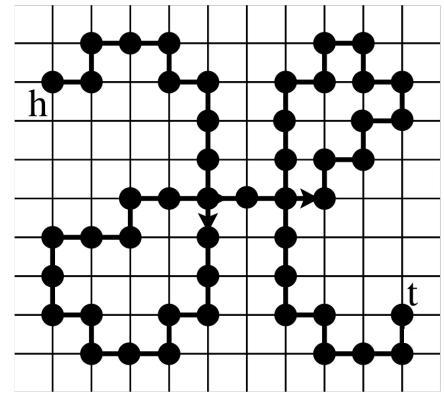
\includegraphics[width=0.45\textwidth]{resideal.jpg}

\caption[Marche aléatoire sur réseau]{Réseau carré montrant la marche aléatoire qui génère une configuration d'un polymère \cite{these}.}
\label{resideal}
\end{center}
\end{figure}

On déduit facilement que pour un degré de polymérisation $N+1$, il y a $Z_{ideal}=z^N$ polymères distincts possibles. Recalculons les résultats fondamentaux concernant la marche aléatoire génératrice du polymère. Ces résultats sont indépendants du réseau qui est un artifice de calcul et ne modifie pas les lois d'échelle. La plupart des modèles numériques n'utilisent pas de maillage. Soit $\textbf{r}$ le vecteur position du marcheur par rapport à l'origine et $b$ la taille d'un pas effectué par le marcheur. Soit $\textbf{r}_n$ le $n$-ième pas effectué, au bout d'un nombre de pas $N$, on a: 

\begin{eqnarray}
\textbf{r} = \sum_{n = 1}^{N} \textbf{r}_n
\end{eqnarray}

Pour la marche aléatoire idéale, il n'y a pas de corrélation entre les différents pas, ce qui mathématiquement se traduit par $\left<\textbf{r}_i \cdot \textbf{r}_j\right> = \delta_{i,j} b^2$. Ce qui implique les relations suivantes:

\begin{eqnarray}
\left<\textbf{r}\right>\text{} = \sum_{n = 1}^{N} \left<\textbf{r}_n \right>\text{} =\text{} 0 \text{ }, \text{} \left<\textbf{r}^2\right> \text{}= \sum_{i = 1}^{N} \sum_{j = 1}^{N} \left<\textbf{r}_i \cdot \textbf{r}_j\right> \text{}= \sum_{i = 1}^{N} \left<\textbf{r}_i^2\right> \text{}= b^2 N
\label{rdmwalk}
\end{eqnarray}

 Puisque la valeur moyenne de $\textbf{r}$ est nulle, on estime le comportement de la distance entre les extrémités (distance bout-à-bout) moyenne du polymère en prenant la racine carré de la valeur moyenne de $\textbf{r}^2$. Comme le montre l'équation \ref{rdmwalk} la taille du polymère sera proportionnelle à $N^\frac{1}{2}$.\\
 
 Une estimation correcte de la taille du polymère est obtenue en considérant le rayon de giration $R_g$. Il est défini de la manière suivante en notant $\textbf{r}_{CM}$ la position du centre de masse du polymère :
 \begin{eqnarray}
R_g^2\text{}=\text{}\frac{1}{N}\sum_{n = 1}^{N} \left<(\textbf{r}_n-\textbf{r}_{CM})^2\right>
\label{equ}
\end{eqnarray}
 Avec $\textbf{r}_{CM}=\frac{1}{N}\sum_{n = 1}^{N} \textbf{r}_n$, ou encore, de manière équivalente: 
  \begin{eqnarray}
R_g^2\text{}=\text{}\frac{1}{2N^2}\sum_{i,j}^N \left<(\textbf{r}_i-\textbf{r}_{j})^2\right>
\label{equbthnth}
\end{eqnarray}
 
 \noindent L'équivalence s'obtient en développant les termes des deux expressions et en les identifiant.\\


On va appliquer la dernière partie de l'équation \ref{rdmwalk} pour la marche aléatoire à l'équation \ref{equ} du rayon de giration en notant le fait qu'on effectue une marche aléatoire de $|i-j|$ pas pour aller du monomère $i$ au $j$ dans l'expression $\left<(\textbf{r}_i - \textbf{r}_j)^2\right>$.

\begin{gather}
R_g^2\text{}=\text{}\frac{1}{2N^2}\sum_{[|i-j|]} |i-j| b^2=\text{}\frac{1}{N^2}\sum_{[i>j]} |i-j| b^2\nonumber \\
=\text{}\frac{b^2}{N^2} \sum_{i=1}^N \sum_{j=1}^{i} j \\
 = \text{}\frac{b^2}{N^2}[\frac{1}{2}(\frac{N(N+1)(2N+1)}{6}+\frac{N(N+1)}{2})]\nonumber
\label{equationgyr}
\end{gather}

En prenant la limite $N \gg 1$ dans l'équation précédente, on obtient la loi d'échelle à laquelle le rayon de giration obéit:
\begin{eqnarray}
R_g^2\text{}\sim\text{}\frac{b^2}{6}N \Rightarrow R_g\propto N^{\frac12}
\end{eqnarray}

La distance bout-à-bout et le rayon de giration obéissent à la même loi d'échelle et sont caractéristiques de l'expansion spatiale du polymère.\\


Revenons à notre modèle sur réseau afin d'établir une équation différentielle sur la probabilité, $P(\textbf{r},N)$, du $N$-ième monomère d'être en $\textbf{r}$ (avec le premier monomère à l'origine). Pour cela, introduisons les z $\textbf{b}_i$  vecteurs les plus proches de la position $\textbf{r}$ pour obtenir:
\begin{eqnarray}
P(\textbf{r},N)= \frac{1}{z}\sum_{i=1}^{z} \left[P(\textbf{r}-\textbf{b}_i,N-1)\right]
\label{eqdifprob}
\end{eqnarray}

On effectue ensuite un développement limité à l'ordre 2 afin d'obtenir une équation différentielle à résoudre sur la probabilité de distribution. Avec pour hypothèse que $\textbf{r}\gg\textbf{b}_i$ et $N \gg 1$.

\begin{eqnarray}
P(\textbf{r}-\textbf{b}_i,N-1)=P(\textbf{r},N)- \frac{\partial P}{\partial N}-  \textbf{b}_{i\alpha} \frac{\partial P}{\partial r_{\alpha} } + \frac12 \textbf{b}_{i\alpha}\textbf{b}_{i\beta} \frac{\partial ^2 P}{\partial r_{\alpha}\partial r_{\beta} }
\end{eqnarray}

En utilisant la convention de sommation d'Einstein, $i$ varie de $1$ à $z$ et $\alpha$ et $\beta$ représentent les coordonnées spatiales. En considérant les résultats suivants:

\begin{eqnarray}
\sum_{i=1}^{z}\textbf{b}_{i\alpha}=0 \text{ },\text{ } \sum_{i=1}^{z}\textbf{b}_{i\alpha}\cdot\textbf{b}_{i\beta} = \frac{b^2\delta_{\alpha,\beta}}{3}
\end{eqnarray}

On obtient l'équation différentielle qui régit la probabilité de distribution de nos monomères:
\begin{eqnarray}
 \frac{\partial P}{\partial N} =   \frac{b^2}{6}\frac{\partial ^2 P}{\partial ^2 \textbf{r}}
 \label{eqdif}
\end{eqnarray}

Cette équation différentielle (\ref{eqdif}) a pour solution avec pour condition initiale $\textbf{r}=0$ quand $N=0$ :
\begin{eqnarray}
P(\textbf{r},N)=\left(\frac{3}{2\pi N b^2}\right)^\frac{3}{2}\exp\left(-\frac{3\textbf{r}^2}{2 N b^2}\right)
\end{eqnarray}

La distribution de probabilité de présence des monomères est donc gaussienne, un polymère idéal est d'ailleurs souvent dit gaussien.\\

Remarquons dors et déjà que le logarithme de la distribution de probabilité donne par définition l'énergie libre du système qui n'est pas sans rappeler celle d'un ressort:
\begin{eqnarray}
F(\textbf{r})= - k_B T \ln(P(\textbf{r},N))= F(0)+\frac{3k_BTr^2}{2Nb^2}
\label{elibre}
\end{eqnarray}
$k_B$ est la constante de Boltzmann. Cette énergie sera utilisée par la suite pour décrire des propriétés dynamiques du polymère.\\



Bien entendu ce modèle est simpliste, un vrai polymère ne peut en aucun cas s'auto-intersecter, il peut ne pas être linéaire...\\

 Traitons le cas d'un polymère qui ne peut s'intersecter lui-même. Les configurations sont alors générées par des marches aléatoires auto-évitantes (Self Avoiding Walks ou SAW). Soit $v_c \propto b^3$ le volume exclusif occupé par un monomère. La probabilité qu'un monomère de la chaîne de volume $R^3$ ne se superpose pas à un autre est $(1-v_c/R^3)$, il y a $\frac{1}{2}N(N-1)$ paires de monomères. La probabilité totale de non superposition est donc:
 \begin{eqnarray}
P_{ns}(N)= \left(1-\frac{v_c}{R^3}\right)^{\frac{N(N-1)}{2}} = \exp\left[\frac{N(N-1)}{2}\text{ }\ln\left(1-\frac{v_c}{R^3}\right)\right]
\end{eqnarray}

La probabilité de distribution d'une SAW est donc le produit des deux probabilités précédentes, ce qui donne dans la limite $N \gg 1$, $R \gg v_c$:
\begin{eqnarray}
P_{SAW}(R,N)=P_{ns}(N) P(R,N)=\exp\left[-\frac{3R^2}{2 N b^2}-\frac{v_cN^2}{2R^3}\right]
\end{eqnarray}

La taille caractéristique du polymère est alors donnée par la valeur $R^*$ qui maximise la probabilité de distribution, d'où:

\begin{gather}
\frac{\partial P_{SAW}(R,N)}{\partial R} \Huge{|} _{R=R^*}=0 \nonumber\\
\Rightarrow \frac{3R^{*2}}{Nb^2}-\frac{3v_cN}{2R^{*4}} =0 \\
\Rightarrow R^* \propto N^\frac{3}{5}\nonumber
\end{gather}


La taille caractéristique du polymère croit donc plus rapidement avec le nombre de monomères que dans le cas idéal précédent. L'exposant 3/5 trouvé est très proche de l'exposant de Flory, $\nu=0.588$, qui fait consensus parmi les différentes simulations numériques. \\


Le cas de la chaîne auto évitante est adapté aux polymères dilués en solution. Le modèle de la chaîne idéale décrit paradoxalement très bien un contexte de polymères en forte concentration en contacte les uns des autres. En effet les termes de volumes exclus s'appliquent pour le polymère aussi bien pour sa propre chaîne que pour la présence de chaînes voisines. L'espace précédemment libre est occupé, le volume exclu apporte une contribution énergétique uniforme dans tout l'espace. Les termes de volumes exclus se compensent donc tous, ce qui permet de se retrouver uniquement avec la contribution d'une chaîne idéale.

Comparons ces prédictions théorique à nos résultats numériques.

\subsubsection{Résultats numériques}
Pour tous les résultats que nous présentons, ici et par la suite, les barres d'erreurs sur la moyenne d'une valeur $A$ sont calculées avec l'équation \ref{errorbar}, $M$ étant le nombre de mesures de la valeur $A$.

\begin{eqnarray}
\sigma=\sqrt{\frac{\left<A^2\right>-\left<A\right>^2}{M}}
\label{errorbar}
\end{eqnarray}

De plus quand nous parlerons de la taille $N$ d'un polymère, nous parlerons d'un polymère ayant une chaîne comprenant $N$ grains. Il y a donc $N$ monomères consécutifs pour les modèles simples. Pour le modèle structuré, nous avons choisi de le symétriser (pour pouvoir par la suite redéfinir une des extrémité à laquelle on va appliquer une force). On a alors un nombre impair $N$ de grains formant la chaîne et $(N-1)/2$ grains latéraux.\\


Dans cette partie concernant la statique des polymères, nous avons observé les valeurs de la distance bout-à-bout et du rayon de giration pour des polymères laissés libres d'évoluer sans contraintes dans un milieu vide (Les interactions avec le solvant demeurent). Nous avons étudié en plus de notre système structuré, des polymères linéaires dont un polymère idéal (les seuls potentiels utilisés sont LJ et FENE uniquement pour les liaisons, l'interpénétration est possible entre grains non liés) et un polymère présentant des volumes exclus \footnote{Modèles réalisés par Gaël Radou lors d'un stage de Master 2 avant mon arrivée au laboratoire.}. Les valeurs des exposants caractéristiques sont légèrement supérieures en raison de la taille finie des modèles. En ce qui concerne notre modèle, nous nous attendons aussi à une valeur plus élevée. En effet les même sources d'augmentation sont présentes. De plus, la présence d'un grain latéral sur le squelette linéaire va augmenter la rigidité de notre polymère. Cette rigidité supplémentaire va augmenter les effets de taille fini. Le squelette sera alors plus longiligne, ce qui aura pour effet d'augmenter plus fortement sa taille effective lorsque $N$ croît. Comme le montre la figure  \ref{statiquenum}, dans le cas d'un polymère idéal, pour la distance bout-à-bout comme pour le rayon de giration, on approche la valeur théorique de $R\propto N^\frac{1}{2}$ par le haut ($R\propto N^{0.529}$ et $R_G\propto N^{0.512}$ respectivement). Pour le polymère linéaire avec volumes exclus, on trouve des valeurs de $\nu$, l'exposant de Flory, plus élevées ($R_G \propto N^{0.639}$) pour les raisons que nous avons avancées et ces valeurs sont encore plus augmentées dans le cas du polymère structuré ($R\propto N^{0.706}$ et $R_G \propto N^{0.697}$). \\


\begin{figure}[H]
\begin{center}
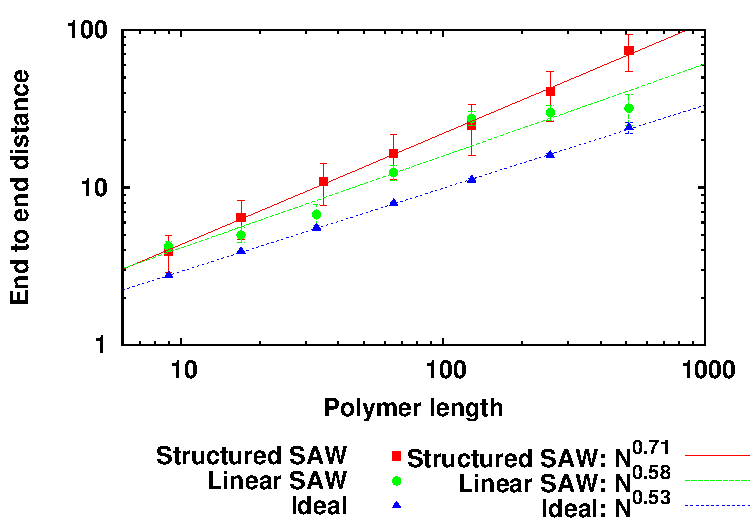
\includegraphics[width=0.9\textwidth]{endtoenddistance.pdf}

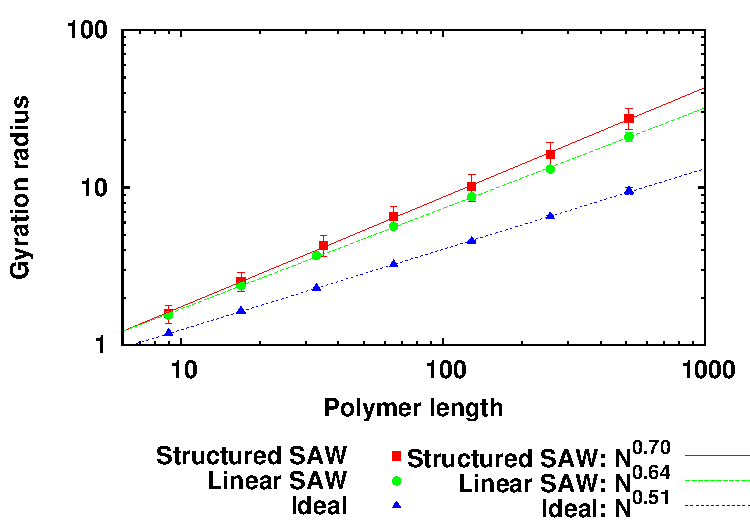
\includegraphics[width=0.9\textwidth]{gyration.pdf}

\caption[Résultats numériques: caractéristiques statiques.]{En haut: évolution de la distance bout-à-bout du polymère. En bas: évolution du rayon de giration du polymère. Des effets de tailles finies, amplifiés par une rigidité accrue dans le cas du polymère structuré, entraînent une estimation surévaluée des exposants prévus, mais ces derniers sont en bon accord avec la théorie. D'un point de vue statique, les différents modèles de polymères ont un comportement tout à fait normal.}
\label{statiquenum}
\end{center}
\end{figure}

\subsection{Dynamique des polymères}
\subsubsection{Théorie}

Nous allons maintenant proposer un modèle permettant d'aborder la dynamique d'une chaîne. Il s'agit du modèle de Rouse \cite{Rouse1953} (Figure \ref{rouse}). Comme nous l'avions signalé, l'énergie libre d'un polymère idéal présente les caractéristiques d'un potentiel harmonique de type ressort (cf: équation \ref{elibre}), ce qui justifie cette modélisation.

\begin{figure}[H]
\begin{center}
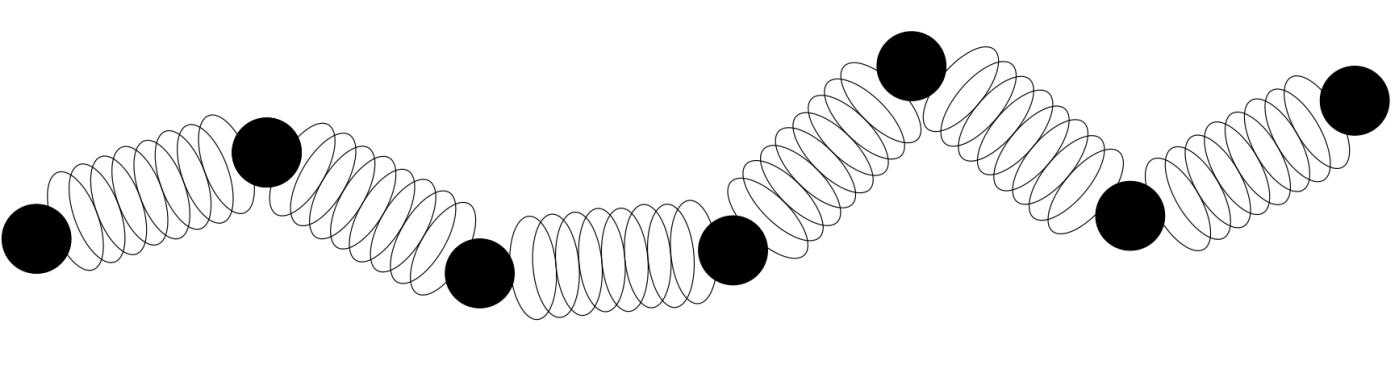
\includegraphics[width=0.8\textwidth]{rouse.jpg}

\caption[Modèle de Rouse]{Modélisation du polymère par une chaîne d'oscillateurs \cite{these}, appelé modèle de Rouse.}
\label{rouse}
\end{center}
\end{figure}

Le polymère est modélisé par une chaîne d'oscillateurs (de type billes/ressorts). Physiquement, le ressort ne représente pas une liaison entre monomères mais plutôt une partie du polymère assez longue pour que la statistique gaussienne puisse lui être appliquée. De l'équation \ref{elibre} obtenue précédemment on déduit l'énergie élastique du ressort connectant les billes $n$ et $n+1$ séparées par une distance d'équilibre moyenne $b$:


\begin{eqnarray}
F_{n,n+1} = \frac{3 k_B T}{2} \frac{(\textbf{r}_{n+1}-\textbf{r}_n)^2}{b^2}
\end{eqnarray}

Nous nous plaçons dans des conditions simples en modélisant l'effet du solvant par un simple terme de frottement visqueux (ou Stokes drag), la trajectoire est donc donnée par l'équation de Langevin ( \ref{langevin}). De plus, les dimensions nanométriques du systèmes impliquent un nombre de Reynolds\footnote{Le nombre de Reynolds est le rapport des échelles de temps caractéristiques inertielles et visqueuses.} très faible. On va donc négliger les termes inertiels dans l'équation de Langevin qui s'écrit ici:

\begin{eqnarray}
\large{
\frac{d \textbf{r}_n}{dt} =  \frac{3k_BT}{\nu_n b^2}( \textbf{r}_{n+1} +\textbf{r}_{n-1} -2\textbf{r}_n )  + \textbf{g}_n}
\end{eqnarray}

On va résoudre cette équation en prenant $n$ comme variable continue.

\begin{eqnarray}
\large{
\frac{d \textbf{r}}{dt} =  \frac{3k_BT}{\nu b^2}\frac{\partial ^2 \textbf{r}}{\partial  n^2} + \textbf{g}_n}
\end{eqnarray}

Avec les conditions limites $\frac{\partial  \textbf{r}}{\partial  n}=0$ en bouts de chaîne, on peut résoudre le système en le séparant en plusieurs modes à  partir de coordonnées normalisées: 
\begin{eqnarray}
\textbf{x}_p= \frac{1}{N} \int_0^N \cos \left(\frac{n\pi p}{N}\right) \text{ }\textbf{r}(n,t)\text{ } dn \text{ , } \frac{d \textbf{x}_p}{dt} =  -\frac{k_p}{\nu _p} \textbf{x}_p + \textbf{g}_p
\end{eqnarray}



\begin{eqnarray}
\nu_0=  N \nu \text{ , } \nu_p= 2 N \nu  \text{ , }  k_p=\frac{6k_BT\pi^2 p^2}{N b^2}  \text{ , }  \left<\textbf{g}_{p\alpha}(t) \cdot \textbf{g}_{q\beta}(t')\right> = 2\delta_{p,q} \delta_{\alpha ,\beta} \frac{k_BT}{\nu_p} \delta(t-t')
\end{eqnarray}

En travaillant dans la nouvelle base orthogonale, on peut montrer que:


\begin{eqnarray}
\left<(\textbf{x}_{0}(t)-\textbf{x}_{0}(0))_\alpha \cdot (\textbf{x}_{0}(t)-\textbf{x}_{0}(0))_\beta \right> = 2 \delta_{\alpha ,\beta} \frac{k_BT}{N\nu}t
\end{eqnarray}

\begin{eqnarray}
\left<\textbf{x}_{p\alpha}(t) \cdot \textbf{x}_{q\beta}(0)\right> = 2\delta_{p,q} \delta_{\alpha ,\beta} \frac{k_BT}{k_p} \exp\left(-\frac{t}{\tau_p}\right) \text{ , } \tau _p = \frac{\nu N^2 b^2}{3\pi^2p^2k_BT}
\end{eqnarray}

La distance bout-à-bout et le rayon de giration sont des combinaisons linéaires des $\textbf{x}_p$ et sont donc assujettis  au temps de relaxation le plus long, $\tau_1$ qui obéit à la loi d'échelle : $\tau_1 \propto N^2$. De même la position du centre de masse est donnée par $\textbf{x}_0$, ce qui permet d'en déduire le coefficient de diffusion du polymère:


\begin{eqnarray}
\left<(\textbf{r}_{CM}(t)-\textbf{r}_{CM}(0))^2\right>=\frac{6 k_B T}{N \nu} t = 6 D_R t
\label{fluctudissip}
\end{eqnarray}




L'équation précédente (\ref{fluctudissip}) traduit le théorème de fluctuation dissipation  en prenant en compte $N \nu$, le coefficient de Stokes global du polymère. Le temps de relaxation peut également être vu comme le temps mis par le centre de masse pour parcourir sa longueur.

 Le temps nécessaire au parcours d'une certaine distance est indépendant de la présence d'interactions entre monomères (chaîne idéale ou SAW), mais la longueur du polymère dépend des conditions du modèle. On a alors $\tau \propto \frac{R^2}{D}$, soit $\tau \propto N^2 $ dans le cas idéal ou $\tau \propto N^{1+2\nu} $ dans le cas de la marche auto-évitante. 

Expérimentalement, on ne retrouve pas ces résultats car le modèle néglige les interactions hydrodynamiques, des interactions à longue portée entre les monomères via le solvant. La figure \ref{hydrodyninterac} illustre ce phénomène. Le modèle de Rouse complété par l'ajout d'interactions hydro- dynamiques s’appelle le modèle de Zimm \cite{Zimm1956}.


\begin{figure}[H]
\begin{center}
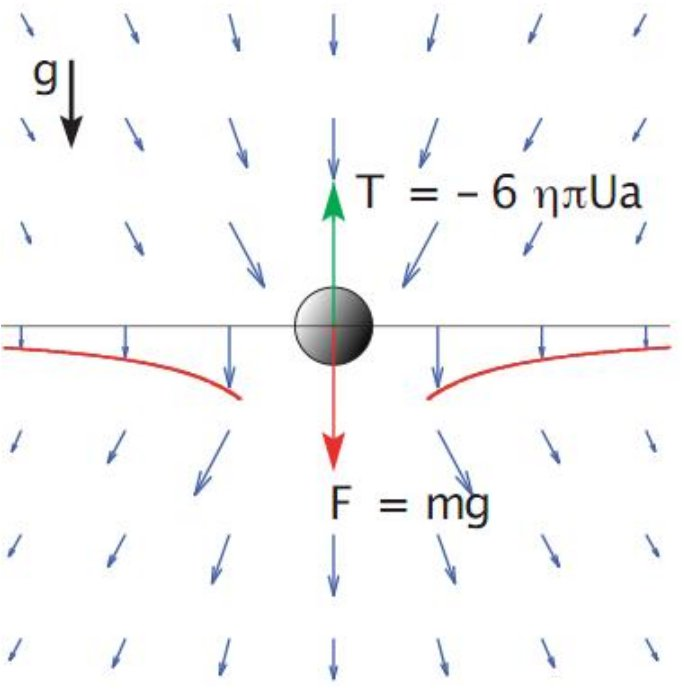
\includegraphics[width=0.4\textwidth]{hydrodyninterac.jpg} 

\caption[Interactions hydrodynamiques]{Mouvement de fluide généré par une bille en chute libre. Pour chaque objet en mouvement, le fluide déplacé génère un champ de vitesse, ces champs de vitesse décroissent en l'inverse de la distance et se superposent, il y a advection des objets par le fluide. Illustration de Bloen Metzger \cite{bloen}.}
\label{hydrodyninterac}
\end{center}
\end{figure}

La compréhension de la dynamique des polymères permet de s'attaquer à l'élaboration de modèles pour la translocation comme nous l'avons vu précédemment.


\subsubsection{Résultats numériques}



Afin de connaître l'évolution de la taille de notre système avec le nombre de monomères nous avons laissé évoluer librement notre polymère pendant un nombre important de pas de dynamique moléculaire (jusqu'au milliard pour les chaînes les plus longues). Cela génère un nombre important de configurations du polymère à l'équilibre. Toutefois, ces configurations ne sont pas indépendantes les unes des autres.\\

Pour connaître l'indépendance de nos configurations, nous avons défini une fonction d'auto-corrélation, $G(H,\tau)$ qui dépend d'une observable $H$ et du temps $\tau$ écoulé entre deux mesures de cette observable.
\begin{eqnarray}
G(H,\tau)=\frac{\left<H(t+\tau)H(t)\right> -\left<H(t)\right>^2}{\left<H(t)^2\right> -\left<H(t)\right> ^2}
\end{eqnarray}

Un script en langage C a été utilisé afin de calculer la fonction d'auto-corrélation pour le rayon de giration et la distance bout-à-bout à partir des données brutes générées par LAMMPS. Dans un premier temps la moyenne et la variance de l'observable sont calculées. Ensuite, un balayage avec une fenêtre de largeur glissante est effectué avec plusieurs valeurs de $\tau$ afin de calculer la quantité $\left<H(t+\tau)H(t)\right>$. Un fit exponentiel est alors effectué afin de déterminer un temps de corrélation. La figure \ref{correl} présente $G(R,\tau)$ du rayon de giration et de la distance bout-à-bout pour différentes tailles de chaîne. Une fois ces temps de corrélation défini, nous pouvons nous intéresser à leur évolution en fonction de la taille de notre polymère.

Le fit exponentiel n'est pas toujours parfait, notamment dans la zone des corrélations fortes, mais il a le mérite d'être une bonne définition du temps de corrélation car au bout de 5 $\tau_c$, la corrélation entre les différentes valeurs des mesures que nous avons prises est nulle. On utilise donc ce fit exponentiel pour estimer nos temps de corrélation. 

L'évolution avec la taille du polymère du temps de corrélation ainsi défini a été étudiée pour la distance bout-à-bout et le rayon de giration comme le montre la figure \ref{dyntpscorrel}. Nous trouvons respectivement $\tau_c \propto N^{2.13}$ et $\tau_c \propto N^{2.19}$ pour la distance bout-à-bout et le rayon de giration. Ces valeurs sont très proches de la valeur théorique $\tau_c \propto N^{1+2\nu} \approx N^{2.18}$. Nous avons vu que nos estimations précédentes de $\nu_{static}$ étaient surévaluées à cause des effets de taille finie. En ce qui concerne les propriété dynamiques, ces effets sont inexistants avec un $\nu_{dynamic}$ bien plus proche de la valeur théorique.

\begin{figure}[H]
\begin{center}
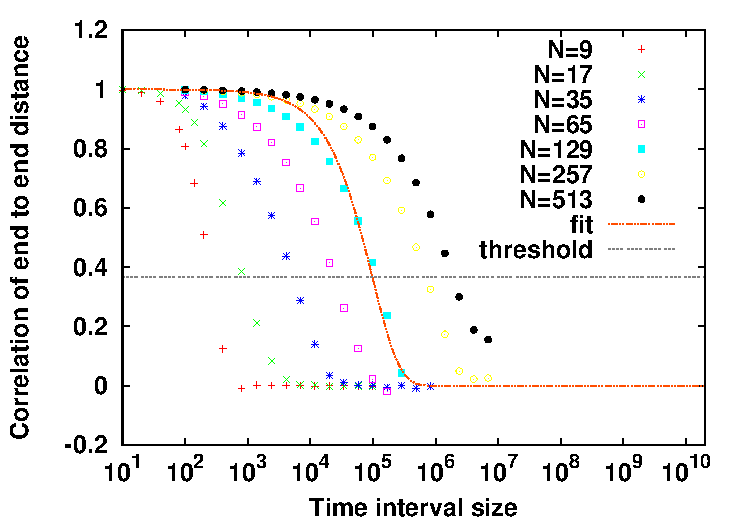
\includegraphics[width=0.9\textwidth]{correlendtoend.pdf}
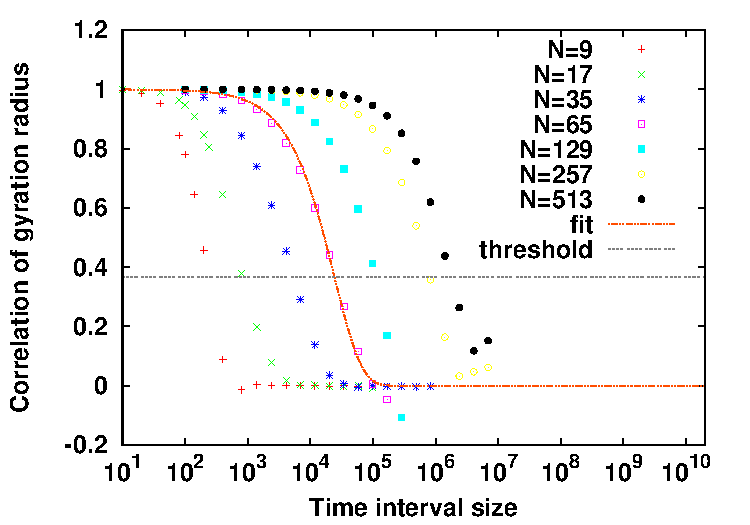
\includegraphics[width=0.9\textwidth]{correlgyr.pdf}

\caption[Résultats numériques: estimation des temps de corrélation]{Auto-corrélation associées à la distance bout-à-bout et au rayon de giration pour différentes longueurs de chaîne du polymère structuré. Le fit exponentiel n'est pas toujours parfait, mais il donne une bonne estimation du temps de corrélation.}
\label{correl}
\end{center}
\end{figure}

\begin{figure}[H]
\begin{center}
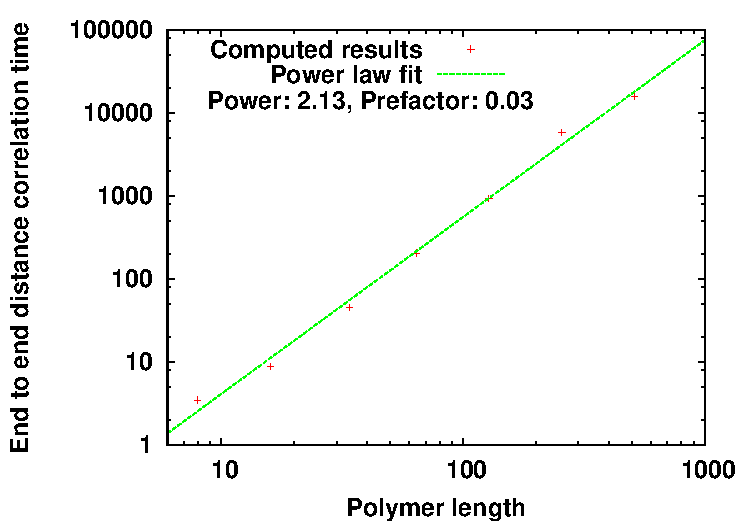
\includegraphics[width=0.9\textwidth]{tpscorrelendtoend.pdf}

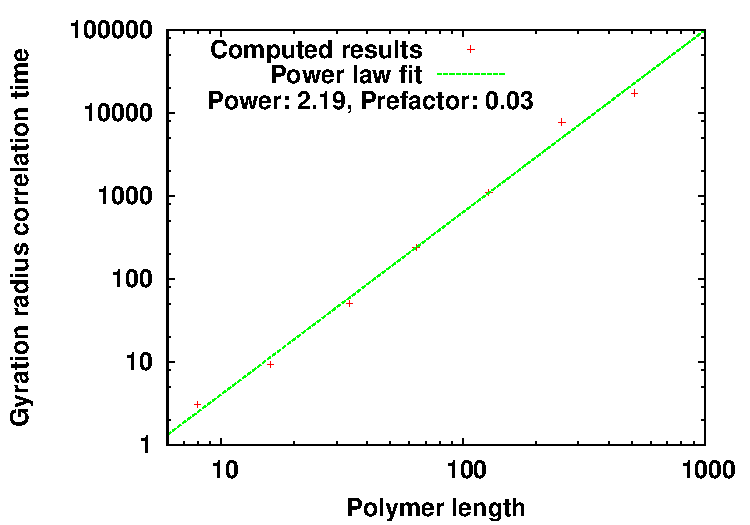
\includegraphics[width=0.9\textwidth]{tpscorrelgyr.pdf}

\caption[Résultats numériques: évolution des temps de corrélation]{En haut: évolution du temps de corrélation de la distance bout-à-bout du polymère. En bas: évolution du temps de corrélation du rayon de giration du polymère. Les valeurs numériques sont très proches de la valeur théorique $\tau_c \propto N^{1+2\nu}$ soit environ $N^{2.176}$. Les effets de taille finie limitent les configurations accessibles et augmente l'exposant de Flory statique $\nu_{static}$, par contre ils ne contraignent pas les fluctuations et les temps nécessaires aux transitions entre configuration, on a donc $\nu_{dynamic}$ bien plus proche de la valeur théorique.}
\label{dyntpscorrel}
\end{center}
\end{figure}


Dans l'étude de la dynamique de notre polymère, nous nous sommes également intéressés au coefficient de diffusion D et à son évolution avec la taille du polymère.

\begin{eqnarray}
\left<(\textbf{r}_{CM}(t)-\textbf{r}_{CM}(0))^2\right>= 6 D_R t
\label{defd}
\end{eqnarray}

Comme le rappel l'équation \ref{defd}, le coefficient de diffusion est lié au déplacement carré moyen du centre de masse. Il ne s'agit pas d'une fonction qui s'évalue à un instant t mais d'une fonction qui s'évalue sur un intervalle de temps. La fonction d’auto-corrélation que nous avons défini précédemment ne peut donc pas être utilisée ici. Nous avons alors fait varier l'intervalle de temps utilisé pour estimer D. On obtient la figure \ref{dexptime}. On remarque que la valeur ainsi évaluée atteint exponentiellement sa valeur réelle de plateau. Le temps caractéristique pour atteindre ce plateau ne dépend pas de la taille de notre polymère. Ce temps ne dépend en effet que d'efforts extérieurs browniens dus à la température. La figure \ref{fluctu-dissip} montre, en accord avec la théorie que D varie bien de manière inversement proportionnelle à la longueur du polymère.

\begin{figure}[H]
\begin{center}
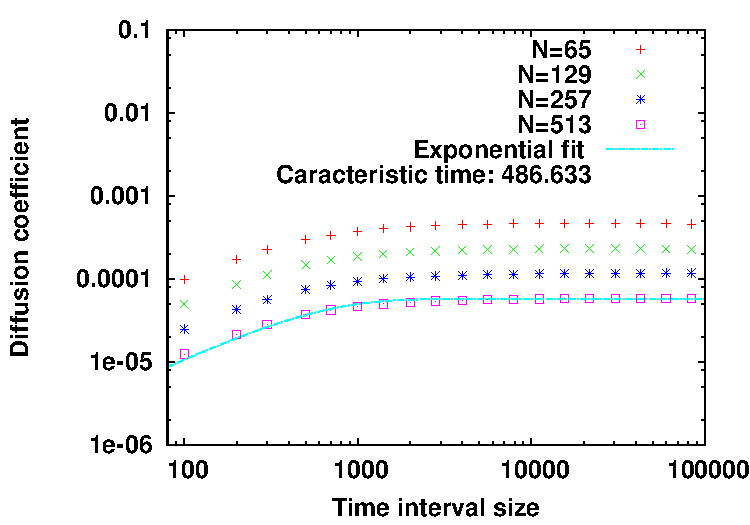
\includegraphics[width=0.8\textwidth]{dexptime.pdf}

\caption[Résultats numériques: estimation du coefficient de diffusion]{Le coefficient de diffusion $D$ est caractéristique de la distance au carrée moyenne parcourue par le centre de masse en un temps $\Delta t$ : $\left<r^2\right> =D\cdot \Delta t$. Nous avons évalué différentes valeurs de $D$ à l'aide de fenêtres glissantes de tailles $\Delta t$ différentes. Pour les petites fenêtres, la valeur de $D$ est fortement sous évaluée. Nous avons remarqué qu'un fit exponentiel de type $D\left(1-\exp\left(-t/\tau\right)\right)$ fonctionne bien et donne quasiment la même valeur de $\tau$ quelque soit le nombre de monomères. $D$ est une caractéristique du centre de masse, il est normal que son amplitude varie avec $N$ car le frottement fluide total évolue avec $N$, et que $\tau$ reste inchangé car il résulte d’efforts extérieurs. Nous avons choisi une fenêtre de taille $5\cdot \tau$ pour évaluer $\left<D(N)\right> $.}
\label{dexptime}
\end{center}
\end{figure}

\newpage

\begin{figure}[H]
\begin{center}
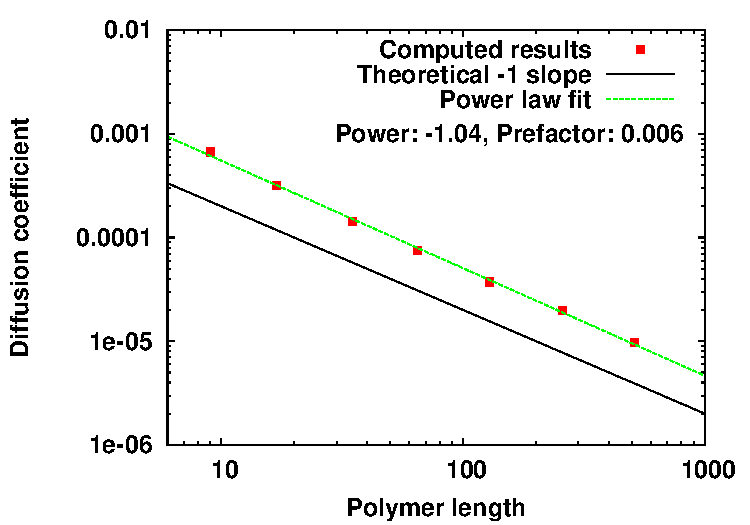
\includegraphics[width=0.9\textwidth]{diffusioncoefficient.pdf}

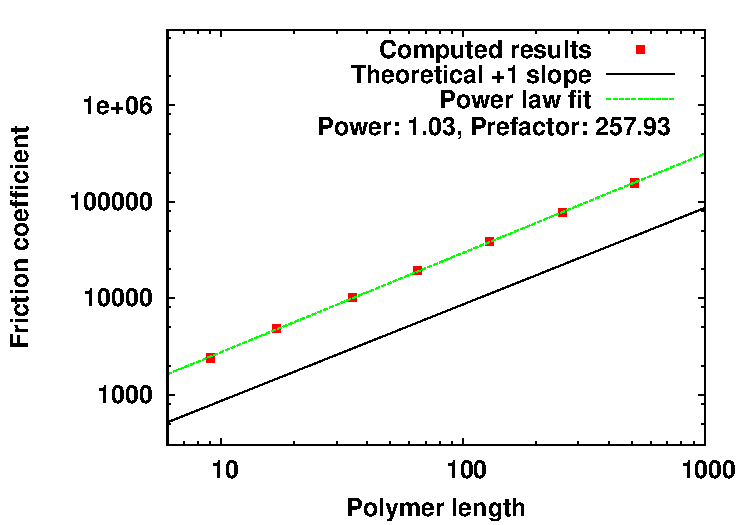
\includegraphics[width=0.9\textwidth]{penteforce.pdf}

\caption[Résultats numériques: évolution des coefficients de diffusion et de friction]{En haut: Décroissance inverse du coefficient de diffusion avec la taille du polymère. En bas: Evolution linéaire du coefficient de friction total avec la taille du polymère.  Le produit des pré-facteurs (1.548 $\epsilon$) donne une bonne estimation de la température du système (défini à 1.5 $\epsilon$). Le théorème de fluctuation-dissipation est ainsi bel et bien vérifié. }
\label{fluctu-dissip}
\end{center}
\end{figure}



Reste maintenant à vérifier le théorème de fluctuation dissipation. Pour cela nous avons imposé une force à une des extrémités du polymère. On observe alors un déplacement linéaire du centre de masse (voir figure \ref{linfrot}). La pente de ce déplacement est calculée pour estimer le coefficient de frottement total du polymère. L'évolution du coefficient de frottement est linéaire. Cette linéarité est attendue car le frottement total est la somme du frottement sur chaque grain. Comme l'illustre la figure \ref{fluctu-dissip}, le calcul de la valeur de ce coefficient de frottement et du coefficient de diffusion sont en accord avec le théorème de fluctuation dissipation.

\begin{figure}[H]
\begin{center}
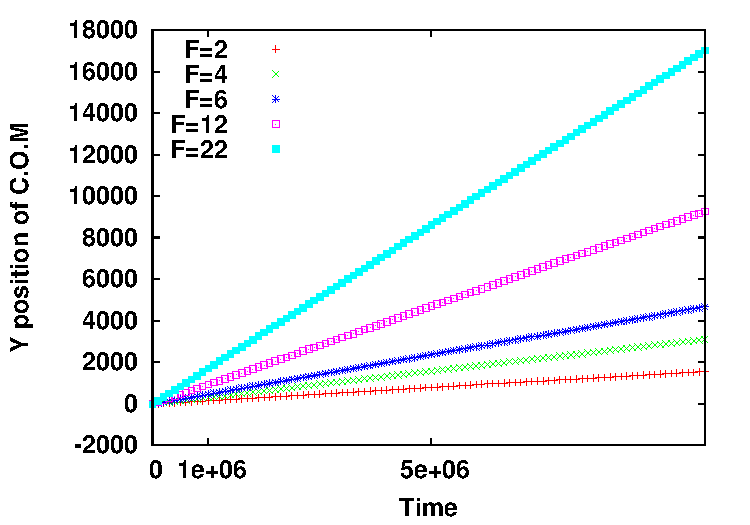
\includegraphics[width=0.8\textwidth]{traction.pdf}

\caption[Résultats numériques: centre de masse en traction]{Evolution de la position, le long de l'axe de traction du centre de masse pour un polymère de longueur N=129. Le centre de masse évolue linéairement dans l'axe de la force imposée à une extrémité du polymère. Cette évolution linéaire permet d'estimer un coefficient de frottement fluide global pour notre polymère.}
\label{linfrot}
\end{center}
\end{figure}


\subsection{Traction du polymère}

Afin de vérifier le théorème de fluctuation dissipation, nous avons imposé une traction à notre polymère. Par la suite, au cours de nos simulations de translocation, le polymère sera également tracté à travers le pore. Il nous a donc semblé intéressant d'exploiter les données ainsi créées.

\subsubsection{Théorie}

En restant dans le cadre du modèle théorique présenté dans la partie précédente, rappelons l'équation du mouvement régissant note polymère:

\begin{eqnarray}
\large{
\frac{d \textbf{r}(n,t)}{dt} =  \frac{3k_BT}{\nu b^2}\frac{\partial ^2 \textbf{r}(n,t)}{\partial  n^2} + \textbf{g}(n,t)}
\end{eqnarray}

Introduisons maintenant une force en bout de chaîne comme le suggèrent Sakaue et al. \cite{Sakaue2012}:

\begin{eqnarray}
\large{
\frac{d \textbf{r}(n,t)}{dt} =  \frac{3k_BT}{\nu b^2}\frac{\partial ^2 \textbf{r}(n,t)}{\partial  n^2} + \textbf{g}_n} + \frac{\textbf{f}(n,t)}{\nu}
\label{equmvt}
\end{eqnarray}

\begin{eqnarray}
\textbf{f}(n,t) = 2f\delta(n)\cdot\textbf{e}_{y} \text{, tel que} \int_{0}^{N} \textbf{f}(n,t) dn = f \cdot \textbf{e}_{y} 
\end{eqnarray}

On a donc une force f appliquée au monomère $n=0$. Par définition, la position du centre de masse peut s'écrire: 

\begin{eqnarray}
\mathbf{r}_{CM}(t) = \frac{1}{N}\int_{0}^{N} \textbf{r}(n,t) dn
\end{eqnarray}

Et sa vitesse s'obtient en dérivant cette expression et en substituant l'équation \ref{equmvt} dans l'intégrale:


\begin{eqnarray}
\textbf{V} = \left<\mathbf{\dot{r}}_{CM}(t)\right> = \frac{f \cdot \textbf{e}_{y}}{N\nu} 
\label{linearfriction}
\end{eqnarray}
Cette équation \ref{linearfriction} justifie la relation linéaire dont nous parlions précédemment (voir figure \ref{traction}).

La déformation de la chaîne peut être calculée en étudiant les modes normaux déjà définis précédemment. On peut déduire la relation suivante:


\begin{eqnarray}
\left<\mathbf{r}(n,t)-\mathbf{r}_{CM}(t)\right> = \frac{Nb^2f}{k_BT}\left[\frac{1}{9}-\frac{1}{3}\left(\frac{n}{N}\right)+\frac{1}{6}\left(\frac{n}{N}\right)^2\right] 
\label{distmonom}
\end{eqnarray}

Et par conséquence pour $L$, l'élongation de la chaîne: 

\begin{eqnarray}
L=|\left<\mathbf{r}(0,t)-\mathbf{r}(N,t)\right> | = \frac{Nb^2f}{6k_BT} 
\end{eqnarray}

On peut également déterminer la propagation de la tension le long de la chaîne du polymère:

\begin{eqnarray}
T(n) = -\frac{3k_BT}{\nu b^2}\left<\frac{\partial  \textbf{r}(n,t)}{\partial  n}\right> \cdot \textbf{e}_{y} = f \left(1-\frac{n}{N}\right)
\end{eqnarray}

$T(n)$ peut être reliée à la taille moyenne $\xi(n)$ du "blob" \cite{Pincus1976} formé en $n$ (voir figure \ref{sakauetraction}):

\begin{eqnarray}
\xi(n) \simeq \frac{3k_BT}{T(n)}
\end{eqnarray}


Bien entendu, ce modèle ne prend pas en compte l'extension maximale finie des liaisons du polymère, il n'a une certaine validité que pour les faibles forces. A forte force, la distance entre monomères atteint l'extension maximale en début de chaîne.

Regardons la taille de la première liaison en utilisant l'équation \ref{distmonom}:

\begin{eqnarray}
\left<|\mathbf{r}(1,t)-\mathbf{r}(0,t)|\right> = \frac{Nb^2f}{3k_BT} \left(\frac{1}{N}-\frac{1}{2N^2} \right) \underset{N\to+\infty}{\longrightarrow} \frac{b^2f}{3k_BT}
\end{eqnarray} 

On remarque que pour une force critique $f_c$, l'extension maximale $b$ est atteinte.

\begin{eqnarray}
f_c=\frac{3k_BT}{b} 
\end{eqnarray} 

Le modèle décris précédemment n'est plus valable dès que $f$ dépasse $f_c$. Considérons la chaîne étirées sur $m$ segments depuis le point d'application de la force, on a alors une extension jusqu'au monomère m où la tension est égale à $f_c$. Pour les $N-m$ segments restants, le modèle précédent demeure pertinent.
L'extension totale est alors la somme des deux segments:

\begin{eqnarray}
L=  m b + \frac{(N-m)b^2f_c}{6k_BT} = mb + \frac{(N-m)b}{2} = \frac{(N+m)b}{2}
\end{eqnarray}

Il est alors possible de relier $m$ à $f_c$ et de déterminer L:
\begin{eqnarray}
f=  N\nu V = f_c + m\nu V \rightarrow m= \frac{f-f_c}{\nu V} = N\left(1-\frac{3k_BT}{fb}\right)
\end{eqnarray}
\begin{eqnarray}
L= Nb\left(1-\frac{3k_BT}{2
fb}\right)
\label{fc}
\end{eqnarray}



\begin{figure}[H]
\begin{center}
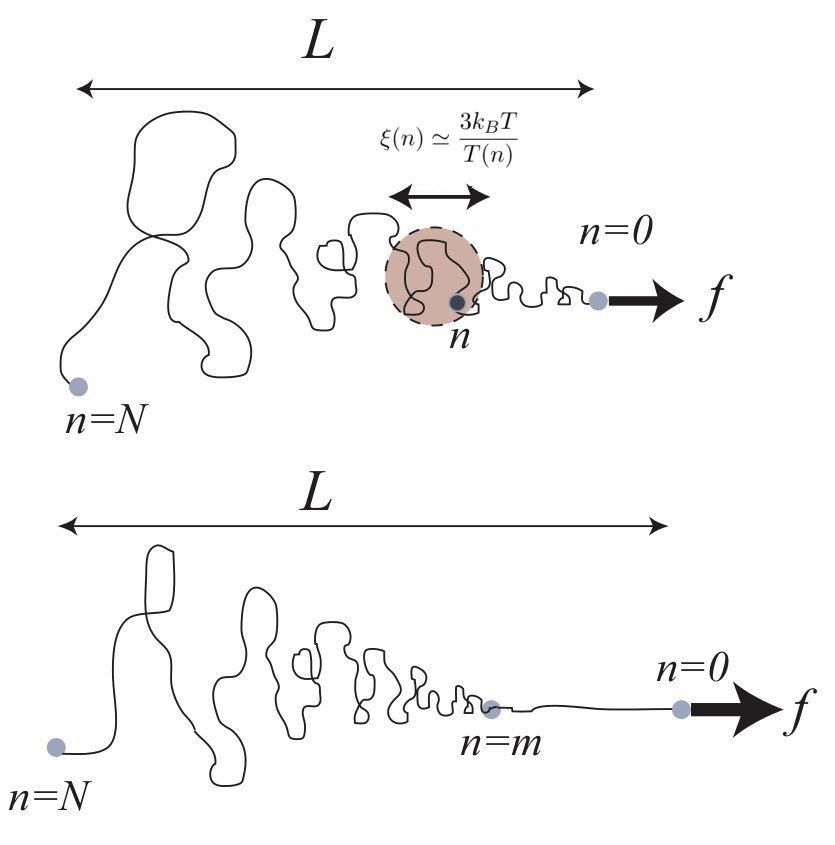
\includegraphics[width=0.6\textwidth]{sakauetraction.jpg}
\caption[Traction d'un polymère]{Modèle simple de l'élongation d'un polymère en traction dans un solvant basé sur un polymère suivant la dynamique de Rouse proposé par Sakaue et al.\cite{Sakaue2012}. En dessous d'une certaine force $f_c$, on observe une légère perturbation de la marche aléatoire du polymère (figure du haut). Le polymère est alors une succession de "blobs" dont la taille dépend de la tension. Lorsque la force de traction est élevée, la chaîne est étirée au maximum jusqu'à ce que la tension retombe à la valeur $f_c$ (en bas).}
\label{sakauetraction}
\end{center}
\end{figure}

Ces résultats théoriques sont valables pour un polymère idéal. Dans notre cas, avec des volumes exclus. Sakaue et al. \cite{Sakaue2012} ne proposent plus de résolution analytique, mais uniquement des raisonnement basés sur des lois d'échelles à faible force (à forte force, les volumes exclus n'interviennent plus sur un polymère étiré).

\subsubsection{Résultats numériques}

Lors de l'évaluation du coefficient de friction de notre polymère, nous l'avons tracté avec une force donnée en bout de chaîne. Précédemment pendant l'évolution du polymère libre, nous avions évalué sa distance bout-à-bout en analysant les coordonnées des monomères de tête et de queues. Ces coordonnées sont maintenant exploitées dans le cas de la traction. 


\begin{figure}[H]
\begin{center}
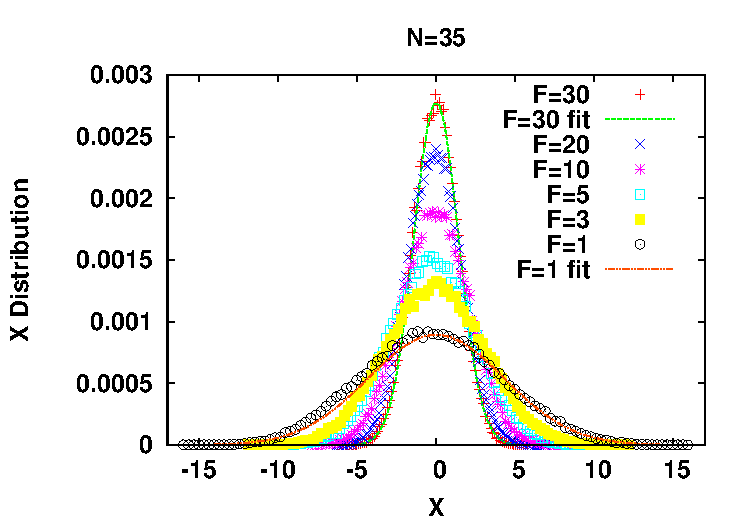
\includegraphics[width=0.5\textwidth]{xdistribution35.pdf}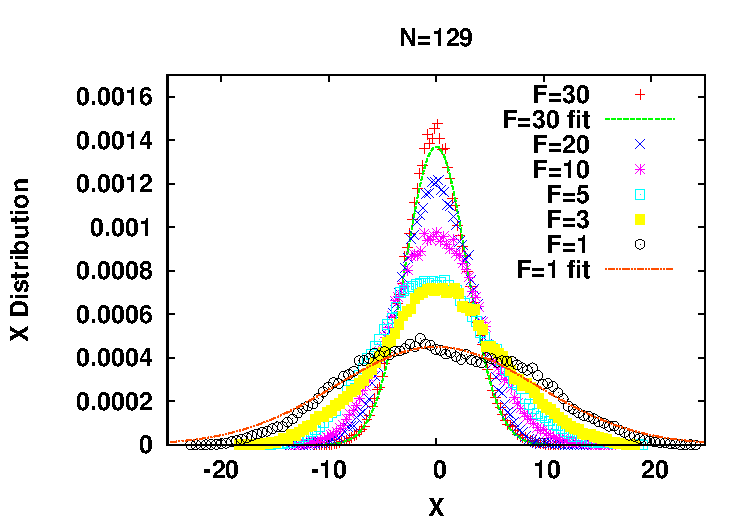
\includegraphics[width=0.5\textwidth]{xdistribution129.pdf}\\
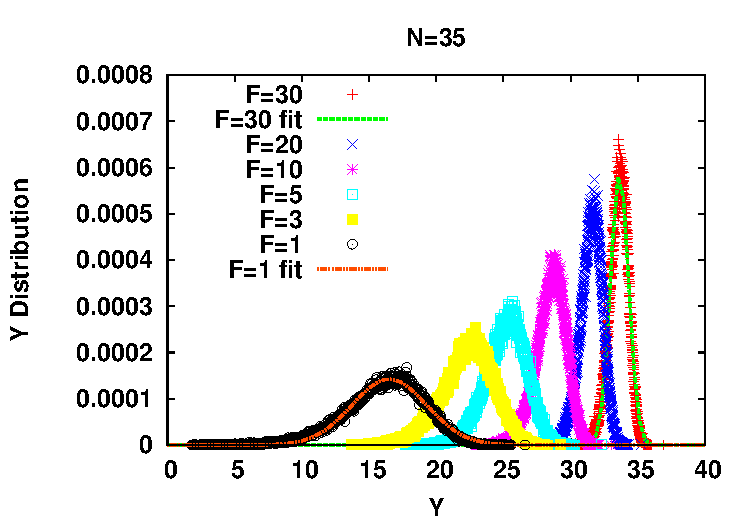
\includegraphics[width=0.5\textwidth]{ydistribution35.pdf}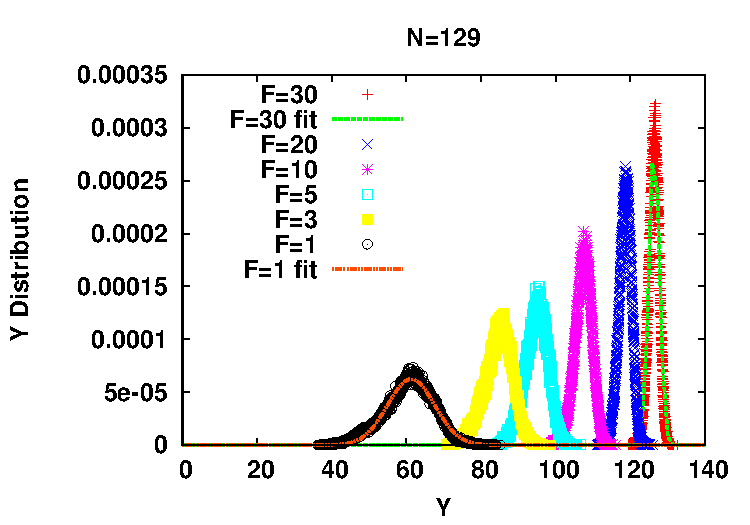
\includegraphics[width=0.5\textwidth]{ydistribution129.pdf}

\caption[Résultats numériques: distributions pendant la traction]{Distribution des composantes perpendiculaires et parallèles à la force de traction de la distance bout-à-bout de notre polymère. Lorsque la chaîne est tractée à forte force (ici dans la direction y), elle s'étire. On voit comme conséquence de cet étirement que selon la coordonnée x (x queue - x tête),  les effets de volumes exclus de la SAW n'interviennent plus. Les distributions perpendiculaires à la force appliquée retrouvent une distribution gaussienne. Cependant la largeur de cette distribution dépend de la force de traction ; plus on tire fort, plus la queue est rabattue vers le centre. En ce qui concerne la direction y, on constate qu'il existe une distribution également gaussienne qui est de plus en plus éloignée de la tête et de plus en plus resserrée au fur et à mesure que la force augmente. }
\label{traction}
\end{center}
\end{figure}

Pour des forces faibles, on observe des distributions qui ne sont pas gaussiennes car les effets des volumes exclus sont importants sur le polymère qui peut se replier car la traction n'efface pas la diffusion. Pour des forces de traction plus élevées, le polymère est étiré et on a alors des distributions qui redeviennent gaussiennes comme le montre la figure \ref{traction}.


L'élongation de notre polymère a été évaluée grâce aux moyennes de la distribution (y queue - y tête) présentées sur la figure \ref{traction}. Cette élongation est comparée au model théorique simple proposé précédemment dans la figure \ref{elongtraction}. Les résultats obtenus sont satisfaisants, car il n'y a pas de paramètre ajustable, et permettent de valider notre modèle de polymère lorsqu'il est tracté.


\begin{figure}[H]
\begin{center}
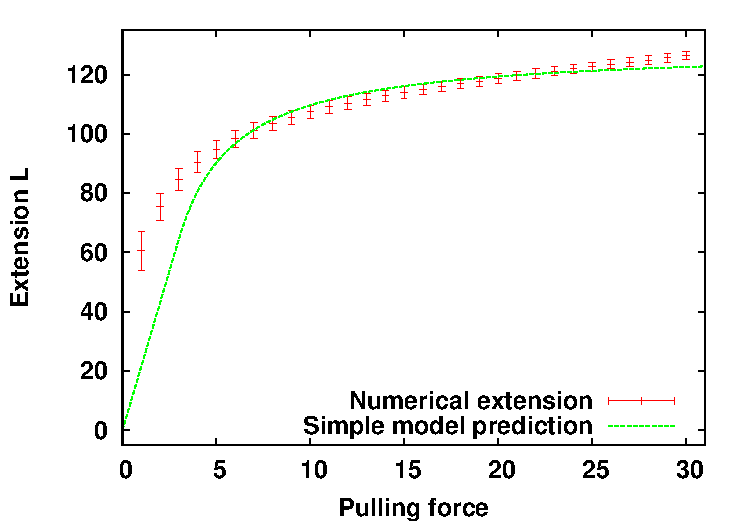
\includegraphics[width=0.9\textwidth]{elongation.pdf}

\caption[Résultats numériques: élongations en traction]{Comparaison de l'extension de notre polymère de taille N=129 en traction avec le modèle simple proposé par Sakaue et al. \cite{Sakaue2012}. A très faible force, on observe une déviation qui est due à la présence de volumes exclus, les grains latéraux ayant tendance à favoriser l'élongation du polymère. A forte force, la comparaison est plus juste, notre extension est légèrement plus élevée, ce qui peut venir de l'utilisation d'un potentiel pour les liaisons présentant une longueur d'équilibre de 1$\sigma$, mais une possibilité d'extension maximale (à force infinie) de 1.5$\sigma$.}
\label{elongtraction}
\end{center}
\end{figure}


Ces prédictions théoriques et résultats numériques semblent être en accord avec les images obtenues expérimentalement lors de la traction d'un ADN marqué par fluorophores \cite{Wirtz1995}.\\

Notre modèle de polymère étant consistant, nous pouvons à présent nous intéresser au problème de la translocation.
